% !TEX root = EUDAQUserManual.tex
\section{Running EUDAQ}

This section will describe running the DAQ system, mainly from the point of view of EUDET-type beam telescope \cite{telescopesWikiUserManual} operated together with \gls{DUT}s.
However, this description can be applied to DAQ system in general.

All executable programs from the different subdirectories are placed inside the \texttt{bin} subdirectory, and should be run from here. They should all accept a \texttt{-h} (or \texttt{--help}) command-line parameter, which will provide a summary of possible different command-line options.

The executable programs mainly split up in two different categories: Processes, which are used for the data acquisition and communicating with the Run Control (DAQ), and utilities, which are used before or after the data taking in order to access the data files (Test, Devel., Tools).
In \autoref{tab:exes}, you will find an overview of the most important EUDAQ executables.

\begin{table}
\centering
\small
\begin{tabular}{ c | l | l | p{4cm}}
  \textbf{Category} & \textbf{Name} & \textbf{Binary}  & \textbf{Description}\\
  \hline			
  \hline			
  DAQ & Run Control & \texttt{euRun} & GUI version, recommended (Sec. \ref{sec:runcontrol}) \\
  DAQ & Log Collector & \texttt{euLog} & GUI version, recommended (Sec. \ref{sec:logcollector}) \\
  DAQ & Online Monitor & \texttt{OnlineMon} & GUI version, recommended (Sec. \ref{sec:onlinemonitor}) \\
  \hline
  Tools & Converter & \texttt{Converter} & CLI, raw data file converter (Sec. \ref{sec:Converter}) \\
\end{tabular}
\caption{Overview of EUDAQ executables: DAQ processes and tools as graphical user interfaces (GUI) or command line interfaces (CLI).}
\label{tab:exes}
\end{table}

\subsection{Preparation}
Some preparation is needed to make sure the environment is set up correctly and
the necessary TCP ports are not blocked before the DAQ can run properly.

\subsubsection{Directories}
EUDAQ expects two directories that will be used to store data files and log files.
These can be directories or symbolic links to other directories.

Firstly, inside the \texttt{eudaq} directory, there should be a directory (or a symbolic link) called \texttt{data}.
This will contain the data files written by the Data Collector, as well as a file containing the last run number,
so that it will continue incrementing even when the DAQ is restarted. 
Secondly, there should be a directory (or symbolic link) called \texttt{logs}.
This will be used by the Log Collector to store log files containing all the log messages received.


\subsubsection{Ports and firewall}
The different processes communicate between themselves using TCP/IP sockets.
If a firewall is running, it may block these connections,
especially if the processes are running on different computers.
If all the processes will be run from the same computer,
then it is probably not necessary to do anything.
If a port is blocked, you will see an error message similar to the following
when attempting to start some programs:
\begin{listing}[]
Are you sure the server is running? - Error 61 connecting to localhost:44000: Connection refused
\end{listing}

The ports can be configured when calling the the processors on the command line (see below), but the default and usually free port numbers are:
\begin{description}

\ttitem{44000}
The Run Contorl listens at this port to get connections with clients (LogCollector, DataCollector, Monitor, Producer). Commands are send, client status are received by RunControl. 

\ttitem{44002}
The Log Collector listens at this port to get connections with clients (RunContorl, DataCollector, Monitor, Producer). Client log messages are received by LogCollector.

\end{description}

If processes will be running on different computers,
then these ports should be opened up in the firewall.
The method for doing this depends on the Operating System used,
and is outside the scope of this manual.


%%%%%%%%%%%%%%%%%%%%%%%%%%%%%%%%%%%%%%%%%%%%%%55
\subsection{Processes}
The DAQ system is made up of a number of different processes that may all be run on the same,
or on different computers. 

\subsubsection{Run Control}
\label{sec:runcontrol}
There are two versions of the Run Control -- a text-based version \texttt{euCliRun} and a graphical version \texttt{euRun} (see \autoref{fig:RunControl}).

\begin{figure}[htb]
  \begin{center}
    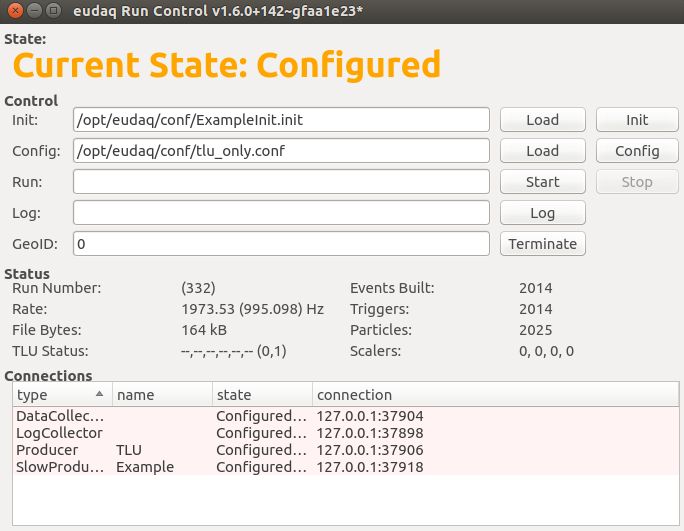
\includegraphics[width=0.8\textwidth]{src/images/RunControl}
    \caption{The Run Control graphical user interface.}
    \label{fig:RunControl}
  \end{center}
\end{figure}

Usually, no command-line option should be needed. 

\paragraph{Finite-State Machine}
\label{sec:fsm}

\begin{figure}
\begin{center}
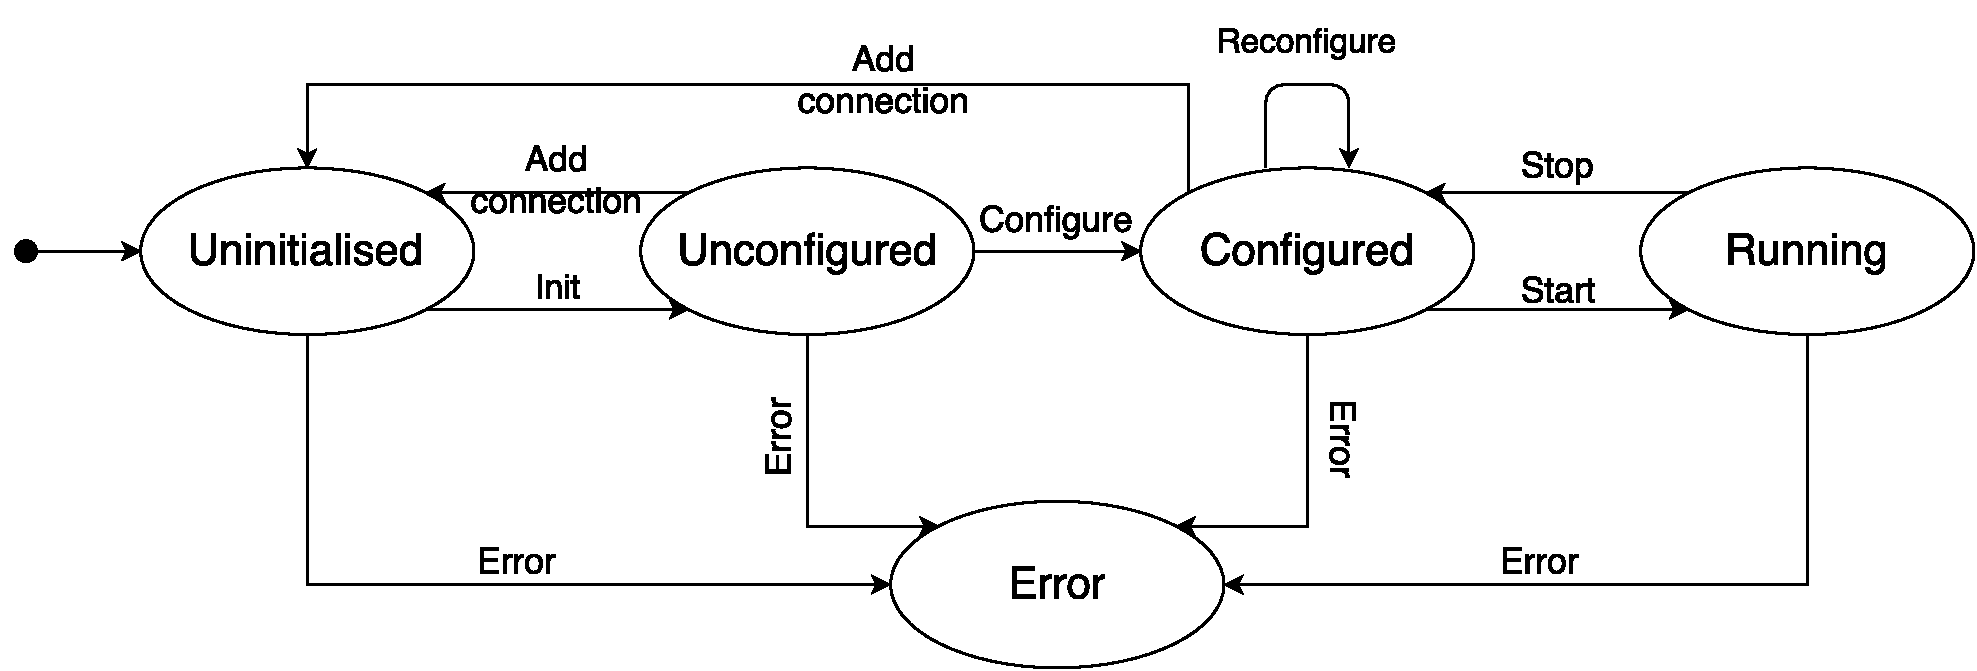
\includegraphics[width=0.9\textwidth]{src/images/fsmv2.pdf}
\end{center}
\caption{The FSM of EUDAQ.}
\label{fig:fsm}
\end{figure}

Since EUDAQ version 1.7, a \gls{FSM} is implemented (see \autoref{fig:fsm}) \cite{Shirokova:2016}.
Each client connected to the Run Control can always be characterized by the current state:

\begin{itemize}
\item UNINITIALISED: the initial state of every client. Initialisation has not been conducted. Available transitions are \texttt{DoInitialise} and \texttt{DoReset}.%
\item UNCONFIGURED: initialisation has already been conducted, but configuration parameters have not been set yet. Available transitions are \texttt{DoConfigure} and \texttt{DoReset}.
\item CONFIGURED: configuration parameters have already been set. Available transitions are \texttt{DoStartRun}, \texttt{DoConfigure} and \texttt{DoReset}.
\item RUNNING: the state of the operating client. For producers it means producing data, the \texttt{OnlineMonitor} are providing plots, the \texttt{LogCollector} is continuing to collect log messages and the \texttt{DataCollector} combines data streams from producers. The only available transition is \texttt{DoStopRun}.
\item ERROR: this state can be used by users in case of errors during configuration, running process, etc. The only available transition is \texttt{DoReset}.
\end{itemize}

The state of RunControl is determined by the lowest state of the connected client (\texttt{LogCollector}, \texttt{DataCollector}, \texttt{Monitor}, \texttt{Producers}) in the following priority: ERROR, UNITIALISED, UNCONFIGURED, CONFIGURED, RUNNING. It means, for example, that even if only one connection is in the ERROR state, the whole machine will also be in that state. This prevents such mistakes as running the system before every component has finished the configuration.

\subsubsection{Log Collector}
\label{sec:logcollector}
It is recommended to start the Log Collector directly after having started the Run Control and before starting other processors in order to collect all log messages generated by all other processes.

\begin{figure}[htb]
  \begin{center}
    \includegraphics[width=\textwidth]{src/images/LogCollector}
    \caption{The Log Collector graphical user interface.}
    \label{fig:LogCollector}
  \end{center}
\end{figure}

Like the Run Control, there are also two versions of the Log Collector.
The graphical version is called \texttt{euLog},
and the text-based version is called \texttt{euCliLog}.

If it is running on the same machine as the Run Control, it should not need any command-line options.
However, if it is running on a different machine, it must be told on which machine the Run Control is running.
\begin{listing}[mybash]
$[./euLog]$ -r tcp://{run_contorl_hostname}:{run_contorl_port}
\end{listing}
The port can also be set using the \texttt{-a \param{port}} option, similar to the Run Control.

\subsubsection{Data Collector}
\label{sec:datacollector}
The Data Collector is the process that collects all the raw data from the Producers,
merges all the connected incoming streams into a single data stream, and writes it to file.
There is only a text-based version called \texttt{euCliDac}.

The command line parttern to startup a DataCollector is:
\begin{listing}[mybash]
$[euCliDac]$ -n {code_name_of_data_collector} -t {runtime_name_of_data_collector} -r tcp://{run_contorl_hostname}:{run_contorl_port} -a tcp://{listening_port}
\end{listing}

Option \texttt{-n} required\\
Option \texttt{-t} required\\
Option \texttt{-r} optional, \texttt{run\_contorl\_hostname} default value: localhost;  \texttt{run\_contorl\_port}  default value: 44000\\
Option \texttt{-a} optional, \texttt{listening\_port} default value is random\\

By default, an example DataCollector \texttt{Ex0DataCollector} is avalible. For example, you may startup a instance of \texttt{Ex0DataCollector} by
\begin{listing}[mybash]
$[euCliDac]$ -n Ex0DataCollector -t my_dc
\end{listing}


It is also possible to run multiple Data Collector instances within
one EUDAQ session. 

If you wish to run several instances of the Data Collector on one
machine, you need to make sure that they listen to different addresses
using the \texttt{-a} option as described above. 
Furthermore, each Data Collector has to write to a different file by including the
\texttt{FilePattern} option in the corresponding section of your
configuration file (also see section \ref{sec:ConfigFiles}):

\begin{listing}[conf]
[DataCollector.my_dc_name]
FilePattern = "{path_to_data_folder}/run$6R$X"
\end{listing}

\subsubsection{Monitor}
\label{sec:onlinemonitor}
The Online Monitor reads the data file written by the Data Collector,
and generates several ROOT histograms that can be useful for online monitoring.
Since it reads the native data file directly, it must be run on the same machine as the Data Collector. (TODO)

\begin{figure}[htb]
  \begin{center}
    \includegraphics[width=0.8\textwidth]{src/images/OnlineMonCorrelations}
    \caption{The OnlineMon showing correlation plots between different
      Mimosa26 planes of the EUDET telescope.}
    \label{fig:OnlineMonPlots}
  \end{center}
\end{figure}

The Online Monitor can be run in one of two modes: online or offline.
In online mode, it connects to the Run Control, so it will know when new runs are started,
and it will automatically open each new data file as it is created.
To run it in online mode, the \texttt{-r} option may be used to assign Run Control, in this example:
\begin{listing}[mybash]
$[./OnlineMon]$ -r tcp://{run_control_hostname}::{run_contorl_port}
\end{listing}
Note: The Online Monitor is working properly on Unix machines..

In offline mode, there is no Run Control,
and it only analyses the data file it is given on the command line usind the \texttt{-f} option. 
An example command line is:
\begin{listing}[mybash]
$[./OnlineMon]$ -f {path_to_data_file}
\end{listing}

\subsubsection{Producer}
\label{sec:testproducer}
For testing purposes, you may use the TestProducer.
This works similarly to a real producer, but does not talk to any real hardware,
instead providing a menu for the user to manually send events.

The ExampleProducer was written to illustrate the writing of a new Producer (see \autoref{sec:Producers}).
However, it will actually generate some example data, and so can also be used for testing purposes.
It works more like a real Producer than the TestProducer,
in that it does not require user intervention to generate each trigger,
and the data generated emulates a simple (but realistic) sensor,
and can be properly converted, and therefore displayed in the Monitor.

\subsubsection{Other/DUT Producer(s)}
If you have a producer for your own hardware (see \autoref{sec:Producers}),
it should also have an option to set the address of the Run Control.


\subsubsection{Python Interface and Wrapper for Core EUDAQ Components}
\label{sssec:pywrapper}
A Python interface is provided for selected EUDAQ components:
RunControl, DataCollector and a Producer, that can be extended on the
Python side. The interface is realized through the \texttt{ctypes}
package that is part of every standard Python installation and
requires the \texttt{numpy} Python package to be installed. The
interface code for all components is located in the
\texttt{main/python} directory.

To use the interface and access the components as Python objects, the
wrapper must be loaded inside your Python script:

\begin{listing}[python]
  #!/usr/bin/env python2 
  execfile('PyEUDAQWrapper.py') # load ctypes wrapper

  prc = PyRunControl() # start run control with default settings
  # wait for more than one active connection to appear
  while prc.NumConnections < 2:
      sleep(1)
  prc.Configure("ExampleConfig") # load configuration file
  while not prc.AllOk:
      sleep(1) # sleep while waiting for all connected producers
  prc.StartRun()
\end{listing}

This little scripts creates a RunControl instance, sends a
configuration to all connected producers, waits for their reply, and
starts a new run. Several more extensive examples for using Python
with EUDAQ are located in the \texttt{python} directory in the main
EUDAQ directory.

%%%%%%%%%%%%%%%%%%%%%%%%%%%%%%%%%%%%%%%%%%%%%%%%%%%%%%%%%%%%%%%55
\subsection{Running the DAQ}

\subsubsection{Starting EUDAQ}\label{sec:STARTRUN}
To start EUDAQ, all of the necessary processes have to be started in the correct order.
The first process must be the Run Control (euRun),
since all other processes will attempt to connect to it when they start up.
Then it is recommended to start the Log Collector,
since any log messages it receives may be useful
to help with debugging in case everything does not start as expected.
Finally, the Data Collector, Producers and Monitor can be started.

\subsubsection{Operating EUDAQ}
Once all the processes have been started, 
and by using the Run Control (see \autoref{fig:RunControl}),
According to the machine state \autoref{sec:fsm}, EUDAQ and all processes can be initialized, configured or re-configured, data taking (runs) can be started and stopped, and the software can be terminated.

\begin{itemize}
\item First, the appropriate initialisation file should be selected (see \autoref{sec:ConfigFiles} for creating and editing init-files). Then the \texttt{Init} button can be pressed,
which will send a initialisation command to all connected processes.

\item Second, the appropriate configuration should be selected 
(see \autoref{sec:ConfigFiles} for creating and editing configurations),
and the \texttt{GeoID} should be verified (see \autoref{sec:GeoID}), before continuing.
Then the \texttt{Config} button can be pressed,
which will send a configuration command
(with the contents of the selected configuration file) to all connected processes.
The full contents of the configuration file will also be stored
in the \gls{BORE} of the data file,
so that this information is always available along with the data.
\item Once all connected processes are fully configured, a run may be started, by pressing the \texttt{Start} button.
Whatever text is in the corresponding text box ("\texttt{Run:}") when the button is pressed
will be stored as a comment in the data file.
This can be used to help identify the different runs later.
\item Once a run is completed, it may be stopped by pressing the \texttt{Stop} button.
Runs will also stop and restart automatically when the data file reaches a threshold in size (by default this is 1~GB).%
\footnote{This is because there is a file size limit of 2~GB for storage on the GRID,
and the processed files can grow bigger than the original native files.}
The threshold size for restarting a run may be configured in the config file (see \autoref{sec:ConfigFiles}).
\item At any time, a message may be sent to the log file by filling in the ("\texttt{Log:}") text box and pressing the corresponding button.
The text should appear in the LogCollector window, and will be stored in the log file for later access.
\item Once the run is stopped, the system may be reconfigured with a different configuration, or another run may be started; or EUDAQ can be terminated.

\end{itemize}

\subsubsection{Init/Config-Files}\label{sec:ConfigFiles}
\texttt{$\ast$.ini}-files for initialisation and \texttt{$\ast$.conf}-files for configuration
are text files in a specific format, containing name-value pairs separated into different sections.
See \autoref{sec:ExampleConfig} for an example file.

Any text from a \texttt{\#} character until the end of the line is treated as a comment, and
ignored.  
Each section in the config file is delimited by a name in square brackets
(e.g. \verb@[RunControl]@).  
The name represents the type of process to which it applies; if there
are several such processes, then they can be differentiated by including the name after a period
(e.g. \verb@[Producer.Example]@).  
Within each section, any number of parameters may be specified,
in the form \mbox{\texttt{Name = Value}}.  
It is then up to the individual processes how these
parameters are interpreted.

The entire contents of the config file will be sent to all processes during the configuration, and
each process will have the appropriate section selected.  
The file will also be attached to the
\gls{BORE}, so that it is available with the data later, even if the original config file is
modified or deleted.


%%%%%%%%%%%%%%%%%%%%%%%%%%%%%%%%%%%%%%%%%%%%%%%%%%%%%%%%%%%%%
\subsection{Other Utilities}
There are a number of other utilities available that are not needed for running the DAQ,
but can be useful for other tasks such as debugging.
The executables are all located in the \texttt{bin} subdirectory.
They should all accept a help (\texttt{-h} or \texttt{--help}) option,
to print a summary of the available options.


\subsubsection{FileChecker}
\label{sec:FileChecker}

This is a small utility that reads raw data files and checks if all events are
readable, can be syncronised using the TLU trigger id and lists which type
of subevents the file contains.

It should be called with list of file paths or run numbers. For any argument
that consist only of numerical digits the file path is constructed by
substituting \texttt{\$6R} in the input pattern (defaults to
``\texttt{../data/run\$6R.raw}'') with the run number padded to 6 digits.

For example:
\begin{listing}[mybash]
$[./FileChecker]$ {6045..6050}
\end{listing}

This would produce the following output.
\begin{listing}[]
run     valid  num_events  contains                   errors                    
------  -----  ----------  -------------------------  ----------------------
  6045   true       13131  MUPIX4,NI,TLU                                        
  6046   true           1  MUPIX4,NI,TLU                                        
  6047   true       14674  MUPIX4,NI,TLU                                        
  6048   true        7776  MUPIX4,NI,TLU                                        
  6049  false           0                             no events in the file.    
  6050  false          -1                             read error. 
\end{listing}


\subsubsection{Converter}
\label{sec:Converter}
The \texttt{Converter} program will read a native data file,
optionally select just a subset of events from the file,
and can then write it out to another file in either the same native format, or a different format.
The most commonly used options are:
\begin{description}
\ttitem{-t \param{type}}
The file type to write out.
The available types are listed below.

\ttitem{-e \param{range}}
Select the specified range of event numbers.

\ttitem{-s}
Try to resynchronize events based on the TLU event number
(see TestReader in \autoref{sec:TestReader}).

\end{description}

The available output file types are as follows:

\begin{description}\phantomsection\label{lst:FileTypes}

\ttitem{native}
The native EUDAQ binary file format, consisting of a serialised stream of
\texttt{DetectorEvent}s, containing the raw data read out from the hardware.

\ttitem{standard}
Like the \texttt{native} format, this is also a serialised stream,
but in this case it contains \texttt{StandardEvent}s,
in which the raw data has been converted into a standard format.

\ttitem{lcio}
The standard \gls{LCIO} file format used by the analysis software.
This type is only available if EUDAQ was compiled with \gls{LCIO} support.

\ttitem{root}
A Root file containing a TTree with the hit pixel information.

\ttitem{text}
A simple text based format (not yet implemented).

\ttitem{mimoloop}
A text based format mimicking the output of the mimoloop program
(from Angelo Cotta Ramusino and Lorenzo Chiarelli at INFN Ferrara).

\end{description}

Although this program can be used to convert a native data file into \gls{LCIO} format,
the more usual (and therefore better tested) way is to use the EUTelescope converter.

\subsubsection{ClusterExtractor}
\label{sec:ClusterExtractor}
This program can be used to quickly extract some clusters from raw data.
It is not as sophisticated as the EUTelescope package, which should be preferred for real analysis,
but it can be useful for doing quick checks.
It will read a native data file, perform a basic clustering,
and then write these clusters to one text file per sensor plane.
The most commonly used options are:
\begin{description}
\ttitem{-p \param{pixels}}
The cluster size in pixels.
It should be an odd number, with 1 meaning no clustering (just pixels over threshold),
3 meaning 3\x{}3 pixel clusters, etc.

\ttitem{-n \param{adcs}}
The noise level (sigma) in ADC units.
This is used to scale the thresholds in terms of the noise.

\ttitem{-s \param{thresh}}
The threshold for seed pixels, in terms of the noise.

\ttitem{-c \param{thresh}}
The threshold for the total charge of a cluster,
in terms of the cumulative noise of all the pixels in the cluster.

\ttitem{-w}
Reports the cluster centre as the weighted average of the pixels,
instead of the position of the seed pixel.

\end{description}

An example use is:
\begin{listing}[mybash]
$[./ClusterExtractor]$ -p 3 -n 3.5 -s 6 -c 10 -w 5432
\end{listing}

This will generate a number of text files named \texttt{runNNN\_eutel\_M.txt},
where \texttt{NNN} is the run number, and \texttt{M} is the sensor plane number.
The format of the output text files is as follows:
\begin{listing}[]
2       2       51487659237
 182    153     126
 241    120     125
3       1       51489095892
 111    67      346
5       1       51491334074
 113    141     171
7       2       51495330212
 252    240     305
 95     170     189
\end{listing}

The first line contains the event number,
the number of clusters, and the TLU timestamp.
Then for each cluster there is one line,
containing the \texttt{x} and \texttt{y} coordinates of the cluster centre,
and the total charge in ADC units.
The cluster lines are prepended with a space to make it easier to scan the file by eye.


\subsubsection{MagicLogBook}
\label{sec:MagicLogBook}
This program is designed to extract as much information as possible from data files and log files,
in order to reconstruct a log book.
Despite its name, it is in fact not magical,
so it is preferable to keep a good log book during running,
rather than relying on this program to generate it later.

The available options are listed below:
\begin{description}
\ttitem{-f \param{fields}}
A list of fields to include in the output, in the form \texttt{name=value},
with multiple fields separated by commas.
If a predefined list is also specified these will be appended to the list.

\ttitem{-s \param{separator}}
The separator to use between fields in the output. The default is a tab character.

\ttitem{-h \param{string}}
A string that appears at the beginning of the header line (with the list of field names),
that can be used to differentiate it from the other lines. The default is an empty string.

\ttitem{-p {name}}
Use a predefined list of fields.
Currently available values are \texttt{normal} and \texttt{full}.

\ttitem{-o \param{file}}
The output filename. By default the standard output is used.

\end{description}

The easiest method of running is to use a predefined list of fields.
There are currently two predefined lists available: \texttt{normal} and \texttt{full}.
If neither of these are suitable, contact the EUDAQ maintainer,
as it may be possible to add more options.

The \texttt{normal} list includes:
\begin{myitemize}
  \item the run number,
  \item the config file name,
  \item the run start time,
  \item for the \glspl{EUDRB}:
  \begin{myitemize}
    \item the mode,
    \item the sensor type,
    \item whether they are running unsynchronized,
    \item the number of boards,
    \item and the firmware version.
  \end{myitemize}
  \item and for the \gls{TLU}:
    \begin{myitemize}
    \item the internal trigger interval,
    \item the AND mask,
    \item the DUT mask,
    \item and the firmware version.
  \end{myitemize}
\end{myitemize}

The \texttt{full} list includes all the values from the \texttt{normal} list,
plus the number of events in the run and the end of run time.
This is because these values can only be known by reading
the whole data file to the end, which is slow, especially for large data files.

If necessary, other information is available using custom fields,
although the syntax for these is a bit complicated,
since it is designed to be as flexible as possible at specifying any information in the data file.
In the future it may be redefined in order to simplify it if possible.
Therefore it is recommended to use a predefined list of fields where possible.
Custom fields are specified as a comma separated list of items in the form \texttt{name=value},
with the name being what will appear on the header line of the output,
and the value specifying what exactly to extract from the file.
The possible values are illustrated below, although not exhaustively:

\begin{mydescription}
  \ttitem{events$^\ast$} The number of events in the run.
  \ttitem{config} The configuration name, or:
  \begin{mydescription}
    \ttitem{config:section:key} The value of the \texttt{key} from the corresponding \texttt{section} in the config
    (e.g. \texttt{config:Producer.EUDRB:NumBoards}).
  \end{mydescription}
  \item{\texttt{bore}, \texttt{tlu}, \texttt{eudrb}, \texttt{eore}$^\ast$:} Something from the \gls{BORE},
  the \texttt{TLUEvent} or \texttt{EUDRBEvent} subevents of the \gls{BORE}, or the \gls{EORE}, respectively:
  \begin{mydescription}
    \ttitem{bore:.Run} The run number
    \ttitem{bore:\param{name}} Otherwise, if the second part does not start with a period, the value of the tag \param{name} is used
    (e.g. \texttt{tlu:DutMask} or \texttt{eudrb:MODE}).
  \end{mydescription}
  \ttitem{log} Something from the log file (not implemented yet).
\end{mydescription}

$^\ast$ items marked with an asterisk require reading the whole data file, and are therefore slow,
especially when large data files are involved.

Note that the \texttt{EUDRBEvent} is now deprecated, having been replaced by the \texttt{RawDataEvent},
but there is currently no way to specify this.

The \texttt{MagicLogBook} command is used as follows:

\begin{listing}[mybash]
$[./MagicLogBook]$ -p normal ../data/*.raw
\end{listing}

This will produce an output similar to the following:
\begin{listing}[]
Run  Config     Mode Det Start                   U P Trg AND  DUT  Tfw Efw
6371 eudet-beam          2009-07-29 07:44:39.535 1 6   0 0xf  0x10 241
6372 eudet-beam          2009-07-29 08:03:05.079 1 6   0 0xf  0x10 241
6373 eudet-m26test       2009-07-30 09:57:45.157 1 6 255 0xff 0x12 241
6374 eudet-m26test       2009-07-30 10:00:45.205 1 6 255 0xff 0x12 241
6375 eudet-m26test       2009-07-30 10:05:38.625 1 6   1 0xff 0x12 241
6376 eudet-m26test       2009-07-30 10:10:00.107 1 6   1 0xff 0x12 241
6379 eudet-m26test       2009-07-30 10:13:05.322 1 6   1 0xff 0x12 241
\end{listing}

Note that the header row has been modified slightly to fit into the page width:
the \texttt{U} should be \texttt{UnSync}, \texttt{P} should be \texttt{Planes},
\texttt{Trg} should be \texttt{TriggerInterval}, \texttt{Tfw} should be \texttt{TLUfw},
and \texttt{Efw} should be \texttt{EUDRBfw}.
The columns \texttt{Mode}, \texttt{Det} and \texttt{EUDRBfw} are missing from the output
due to the fact that this information is now stored in a \texttt{RawDataEvent},
which is not currently accessible with this version of the program.

\subsubsection{Others}
Some programs that are less used (or recently added)
may not be described here.
If they look interesting, you can find out more about them
by running them with the help (\texttt{-h} or \texttt{--help}) option,
or by examining the source code.
